%\begin{frame}
%\frametitle{2 Higgs doublets models for supersymmetry}
%\begin{multline*}
%V(\phi_1,\phi_2)
%= \lambda_1 \left(\phi_1^\dagger\phi_1 - \frac{1}{2} v_1^2\right)^2
%+ \lambda_2 \left(\phi_2^\dagger\phi_2 - \frac{1}{2} v_2^2\right)^2
%\\
%+ \lambda_3 \left[ \left(\phi_1^\dagger\phi_1 - \frac{1}{2} v_1^2\right) + \left(\phi_2^\dagger\phi_2 - \frac{1}{2} v_2^2\right) \right]^2
%+ \lambda_4 \left[ (\phi_1^\dagger\phi_1)(\phi_2^\dagger\phi_2) - (\phi_1^\dagger\phi_2)(\phi_2^\dagger\phi_1) \vphantom{\frac{1}{2}}\right]
%\\
%+ \lambda_5 \left[ \Re(\phi_1^\dagger\phi_2) - \frac{1}{2} v_1v_2\cos\xi \right]^2
%+ \lambda_6 \left[ \Im(\phi_1^\dagger\phi_2) - \frac{1}{2} v_1v_2\sin\xi \right]^2
%\\
%+ \lambda_7 \left[ \Re(\phi_1^\dagger\phi_2) - \frac{1}{2} v_1v_2\cos\xi \right]\left[ \Im(\phi_1^\dagger\phi_2) - \frac{1}{2} v_1v_2\sin\xi \right]
%\end{multline*}
%\end{frame}

%\begin{frame}
%\frametitle{2 Higgs doublets models for supersymmetry}
%\begin{equation*}
%\average{\phi_1}_0 = \frac{1}{\sqrt{2}} \begin{pmatrix}
%0\\v_1
%\end{pmatrix}
%\msep
%\average{\phi_2}_0 = \frac{1}{\sqrt{2}} \begin{pmatrix}
%0\\v_2 \eexp{\im\xi}
%\end{pmatrix}
%\end{equation*}
%
%\begin{equation*}
%\boxed{\tan\beta = \frac{\average{\phi_2}_0}{\average{\phi_1}_0} = \frac{v_2}{v_1}}
%\end{equation*}
%
%\beamercite{Higgs_hunter_guide}
%\end{frame}

%\begin{frame}
%\frametitle{Higgs bosons in the MSSM}
%\begin{center}
%\emph{Minimal Supersymmetric extension of Standard Model}
%
%\vspace{2\baselineskip}
%\begin{tikzpicture}
%\node[anchor=south west, inner sep = 0] at (0,0) {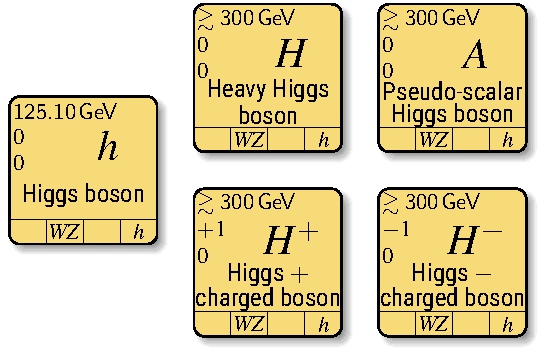
\includegraphics[scale=.7]{\PhDthesisdir/plots_and_images/Particles_tables/MSSM-5Higgs_EN_for_slides.pdf}};
%\node[anchor=south west,inner sep=0, rotate=-30] at (1.35, 2.9) {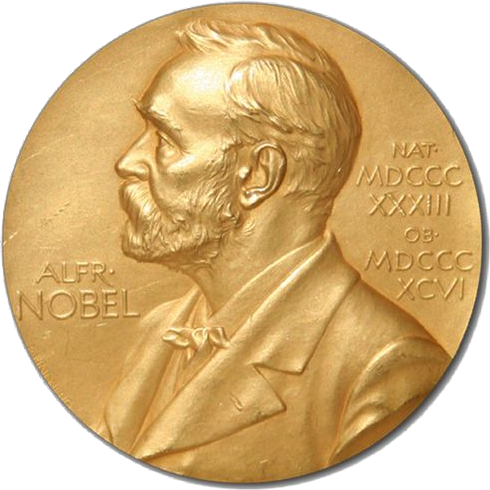
\includegraphics[width=.7cm]{\PhDthesisdir/slides/SM_MSSM_HTT_pheno/MSSM_and_5_Higgs_bosons/nobel-prize-5bf41ed746e0fb00516aa0b3.png}};
%\end{tikzpicture}
%%\manip 2 Higgs doublets $\leadsto$ 5 physical bosons.
%\beamercite{CMS-PAS-HIG-17-020}
%\end{center}
%\end{frame}

\begin{frame}
\frametitle{Higgs bosons in the MSSM}

\begin{minipage}[c]{.475\textwidth}
\begin{center}

\vspace{.5\baselineskip}

\textbf{\small\emph{Minimal Supersymmetric extension of Standard Model}}

\begin{minipage}[c]{.8\textwidth}
\begin{block}{5 Higgs bosons}
\begin{center}
\begin{tabular}{lcc}
light scalar & \higgs & SM or MSSM\\
heavy scalar & \Higgs & MSSM or SM\\
pseudo-scalar & \HiggsA & MSSM\\
$+$ charged & \Higgsplus & MSSM\\
$-$ charged & \Higgsminus & MSSM
\end{tabular}
\end{center}
\end{block}
\end{minipage}

\vspace{.5\baselineskip}

Main parameters:
$m_{\HiggsA}$ and $\tan\beta$.
\end{center}

\beamerlocalcite{CMS-PAS-HIG-17-020}
\beamerlocalcite{Nagashima_BSM}
\end{minipage}
\hfill
\begin{minipage}[c]{.5\textwidth}
\begin{center}
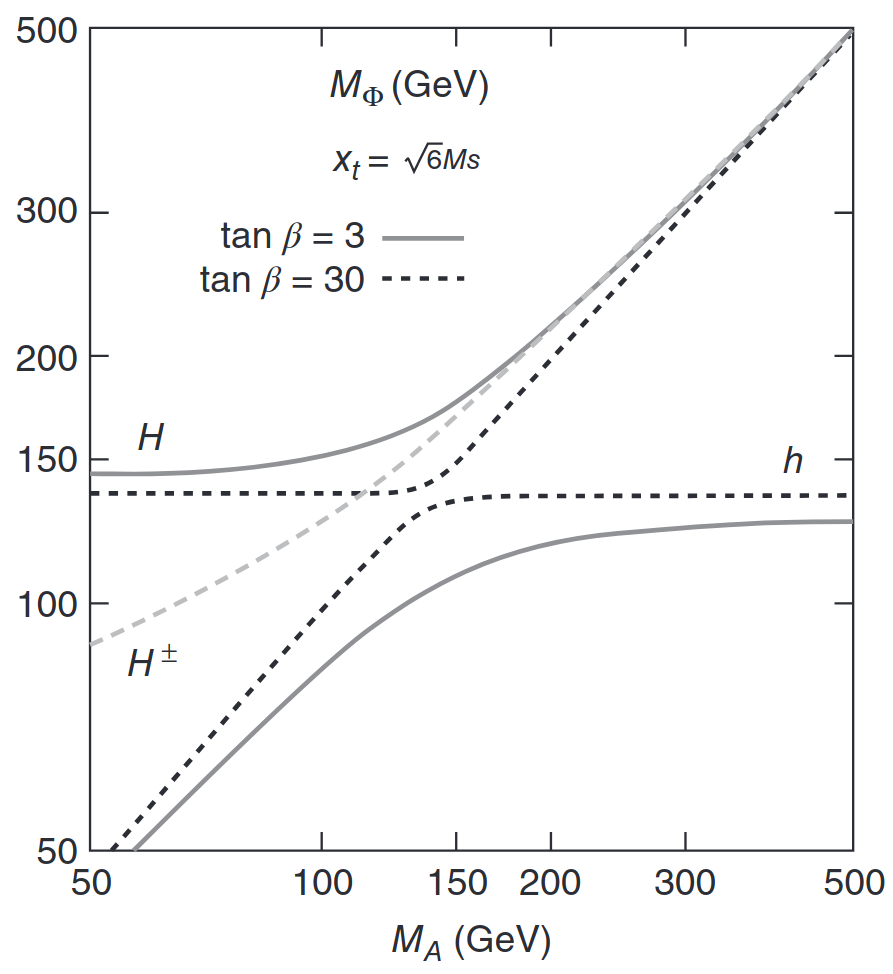
\includegraphics[height=\graphh]{\PhDthesisdir/plots_and_images/from_Nagashima_BSM/fig_1-9.tex}
%\beamercite{Nagashima_BSM}
\end{center}
\end{minipage}
\end{frame}

%\begin{frame}
%\frametitle{Higgs bosons in the MSSM}
%\begin{center}
%
%\begin{tabular}{rccc}
%\toprule
%Couplings & \higgs & \Higgs & \HiggsA \\
%\midrule
%Vector bosons & $\sim1$ & $\sim0$ & $0$\\
%Fermions hauts & $\sim1$ & $\sim-\cot\beta$ & $\cot\beta$ \\
%Fermions bas & $\sim1$ & $\sim\tan\beta$ & $\tan\beta$ \\
%\bottomrule
%\end{tabular}
%\beamercite{Higgs_hunter_guide}
%\end{center}
%\end{frame}
